\experiment{IO System Calls}{11/10/2023}

\section{Aim}
To familiarize the basic I/O ystem calls such as open,close, read and write

\section{Theory}

\subsection{open()}
\subsubsection{Description}
A call to it creates a new open file descriptor, and is used to open a file.
The open() function returns a new file descriptor. Unsuccessful attempt returns -1.

\subsection{read()}
\subsubsection{Description}
It Used to retrieve data from a file stored in a file system.
The value returned is the number of bytes read (or -1 for error)
and the file position is moved forward by this number.

\subsection{write()}
\subsubsection{Description}
It writes data from a buffer to a file/device. The value returned is
the number of bytes written (or -1 for error) successfully.

\subsection{close()}
\subsubsection{Description}
Used to close the file which pointed by file descriptor. Return 0 on success
and -1 on error.

\section{C Program}
\begin{lstlisting}[label={list:c_program:queue}]
#include <stdio.h>
#include <fcntl.h>
#include <sys/stat.h>
#include <string.h>
#include <unistd.h>

int main ()
{
  int fd,fd2;
  char buffer [20]="";
  fd=open ("file1.txt",O_RDWR);
  char data[]="This is a message";
  if(fd!=-1)
  {
    printf("\n File1 Opened");
    write (fd, data, sizeof(data));
    printf("\n Data added to filel: %s\n", data);
    close (fd);
  }
  fd2=open("file2.txt",O_RDWR);
  if (fd2!=-1)
  {
    printf("\n File2 Opened");
    read (fd, buffer,sizeof(data));
    printf("\n Data from file : %s \n",buffer);
    close (fd);
  }
  return 0;
}
\end{lstlisting}

\section{Output}
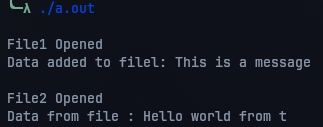
\includegraphics[width=0.75\linewidth]{Cycle_1//Outputs/fileio.png}

\section{Result}
Basic I/O system calls were familiarized and executed successfully